%!TEX root = ../Main.tex

\chapter{General discussion and final remarks}
\label{cha:discussion}
%This section wraps up by showing the relationship and importance of a comprehensive approach to data analysis, from the field, genetics, molecular biology and genomics. I will also remark how the technology and the resources have changed in the last 4 years. As at the references used at beginning where superseded during the PhD. 

%Biology is becoming interdisciplinary

\section{Biology as an interdiciplinary science}

Knowledge from  computer science can be applied to produce software for specific needs, but useful for the comunity

Polyploidy has an extra level of complexity (due to homoeologues), but with the current developments of technology is possible to start getting around them. 



In the case of wheat, new resources had been coming out year after year, and each one helps to put everything in to a context. 

With the plethora of information currently available (See section \ref{lit:wheatResourcers}), it is possible to 


In Chapter \ref{yr15} the integration of different levels of data helped to improve the selection of the candidate SNPs. 
The main criteria for selecting \acrshortpl{snp}  was the\acrshort{bfr} score.
However, thanks to the genetic map from \citet{Wang2014} and the \acrshort{css} scaffolds \citep{Mayer2014}) enabled to confirm that the high scores were in the expected region. 
As the reference genome for wheat improves, the location of SNPs linked to a trait will be easier. 
With a continous reference between two markers flanking a locus and an improve annotation, a more focused set of gene candidates will be possible. 

%However, in the case of introgressions a good reference genome may not be enough to find a gene candidate. 
%This is because the gene may come from a region significantly different to the

\section{The right reference}

The efforts to produce a wheat reference genome had been focused on the \gls{cs} variety. 
\acrshort{cs} is only cultivated as a research line, as it is susceptible to several pathogens and its yield is inferior to modern varieties.  
The reason for \acrshort{cs} to be the selected cultivar to be sequenced as reference is historic: it has long been a variety  for resarch.
\acrshort{cs} was originally picked because it was able to cross with rye. 
It has also been used to produce lines with chromosomic aberrations, useful to find if any particular chromosome is responsible for certain traits \citep{Sears1985}. 


%It is more likely to get relevant results in a more effective way using the latest developments. 


\section{A database to put integrate all the resources. }

\begin{sidewaysfigure}
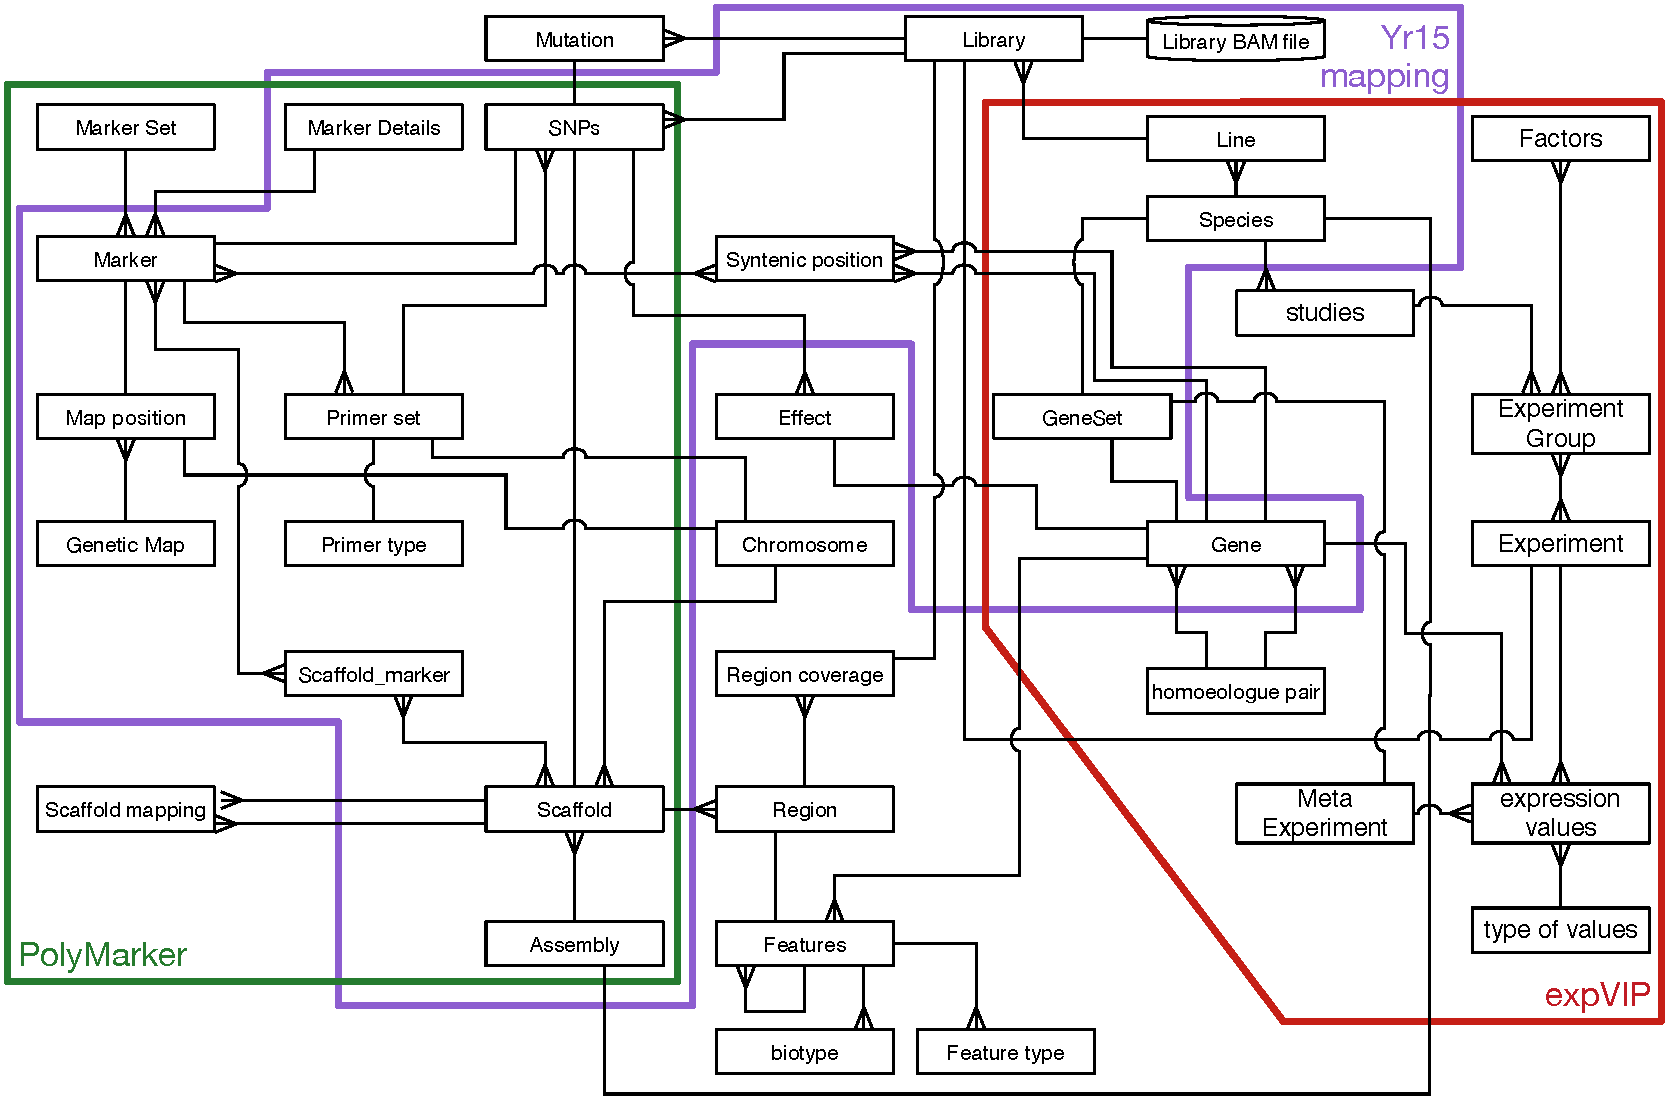
\includegraphics[width=1\textwidth]{Conclusions/Figures/CompleteDatabase.pdf}
\caption{Database integrating all the datasets}
\end{sidewaysfigure}
Integration of the different datasets as used in the project. 
Make the point of the use a GFF File. 

\section{Integration with other services}
Currently, the publicly available wheat resources are scattered as supplemental materials on their corresponding publication or available as ad hoc systems focused on a particular field.
For example ensembl has two different views for every organism: from the genomic point of view and from the expression data. 
The Collaborative Open Plant Omics (COPO; \citealt{Davey2015}) is trying to integrate different sources and types of data by connecting the data providers. 
This approach requires the cooperation of the service providers, which have their own view of what is important. 
I believe that in order to effectively integrate the resources it is necessary to understand how the users are likely to interact with the data.

\section{Side projects}

PolyInDel / . 

\section{Final remarks}

In order to produce bioinformatic software that is powerful and usable it is required an understanding of both: the biological processes to solve and; the computational methods and software development practices.
